\documentclass{article}
\usepackage{graphicx} % new way of doing eps files
\usepackage{listings} % nice code layout
\usepackage[usenames]{color} % color
\definecolor{listinggray}{gray}{0.9}
\definecolor{graphgray}{gray}{0.7}
\definecolor{ans}{rgb}{1,0,0}
\definecolor{blue}{rgb}{0,0,1}
% \Verilog{title}{label}{file}
\newcommand{\Verilog}[3]{
  \lstset{language=Verilog}
  \lstset{backgroundcolor=\color{listinggray},rulecolor=\color{blue}}
  \lstset{linewidth=\textwidth}
  \lstset{commentstyle=\textit, stringstyle=\upshape,showspaces=false}
  \lstset{frame=tb}
  \lstinputlisting[caption={#1},label={#2}]{#3}
}


\author{Matthew Carrano and Breana Leal}
\title{Lab 2: Program Counter Incrementer}

\begin{document}
\maketitle

\section{Introduction}
The purpose behind Lab 2 is to address the ARM's counting and selection capabilities. Counting introduced the assembly of an  Incrementer, the Incrementer uses an adder to allow the program counter to jump to the next instruction in memory. Selection engaged a Mux, a mux allows for the ARM to decide where to jump in memory, either sequentially or to begin branching, based on given inputs.
 
The lab reiterates the use of Verilog modules, testbenches, and simulations for code debugging.

\section{Interface and Implementation}
The incrementer is comprised of an adder. The adder module has two inputs, Ain and Bin, and one output add-out each of [WORD-1:0] length. In Listing 1, the assign statement adds both inputs and assigns the value to the output (add-out). Verilog comprehends higher level programming compared to assembly and does not require gate level details, thus the addition sign is best to use for implementation.   
The mux has two inputs (Ain and Bin) of [SIZE-1:0] length, a single bit selector input, and an output (mux-out) of [SIZE-1:0] length. SIZE is a defined parameter within the mux module of length 8. The assign statement assigns the output (mux-out) a value (Ain or Bin) based on the controlling input (control). Again, Verilog engages the use of the symbols to avoid binary gate logic. 
\Verilog{Verilog code for an Adder.}{code:reg}{../code/1_fetch/adder.v}

\Verilog{Verilog code for a Mux.}{code:reg}{../code/0_common/mux.v}

\section{Test Bench Design}
Listing 3 breaks down cases where 4 is continuously being added to the output after waiting a period of 200ns. Four is passed in for each case to create consistency and following convention. The program counter, therefore will have 4 as the program counter advances. There are two reg (in1 and in2) and one wire (out). 
The mux's testbench has its three reg inputs and one output wire. The mux has a defined parameter of 64 bits. Listing 4 demonstrates four cases when the selector value varies. in1 corresponds to Ain and is selected when con is set to 0. Inversely, in2 corresponds to Bin and is selected when the con is set to 1. Each test is separated by 200ns.

\Verilog{Verilog code for testing an Adder.}{code:regtest}{../code/1_fetch/adder_test.v}

\Verilog{Verilog code for testing a Mux.}{code:regtest}{../code/0_common/mux_test.v}

\section{Simulation}
Figure 1 below is the simulation for the adder testbench. in1 maintains a constant value while in2 is counting by 4s. As expected the output values are incrementing by 4. This result verifies the adder is working.
Figure 2 is the mux testbench results. The first 600 ns have 5 and 8 as in1 and in2 but the out differs based on the con value. When con is set to 0 out is 5 until the time reaches 200ns and con's value changes to 1, also changing out to 8. Cases 1-3 demonstrates the mux's assign statement successes in being able to distinguish between inputs. The remaining time displays the same concept with alternate input values.

\begin{figure}
\begin{center}
\caption{Timing diagram for Adder Test.}\label{fig:regtest}
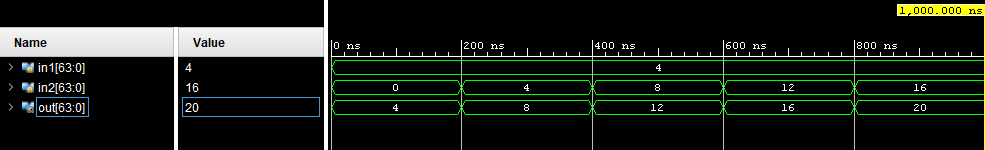
\includegraphics[height=1.25in, width=1.2\textwidth]{../images/adderSim.png}
\caption{Timing diagram for Mux Test.}\label{fig:regtest}
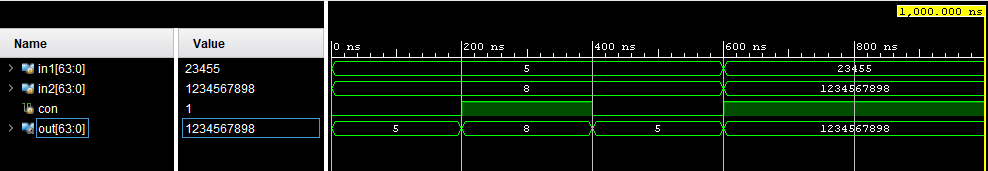
\includegraphics[ height=1.25in, width=1.2\textwidth]{../images/muxSim.png}
\end{center}
\end{figure}



\section{Conclusions}
The coded Verilog files serve as the ARM's fetch section to fulfill its later goal of datapath. Lab 2 introduced an adder and mux to accomplish the program counter's incrementer and branching abilities. The adder added inputs which assigned the summation to its output. The mux had one output selected from multiple inputs based a controlling input. Ultimately, both programs contribute to the ARM's progress in memory addressing.
\end{document} 